% !TEX encoding = UTF-8
% !TEX program = pdflatex
% !TEX root = InformationRetrieval.tex
% !TEX spellcheck = it-IT

% 27 Ottobre 2016
% \subsection{Pesatura dei termini}

Un altro modo per calcolare i pesi dei termini è l'\textbf{inverse document frequency} (\textbf{idf}) che riflette l'importanza di un termine nella collezione dei documenti.

L'idea alla base è che se un termine è presente in tanti documenti, questo sarà meno utile per discriminare i vari documenti e quindi è poco importante anche per il reperimento.

La tipica forma dell'\textit{idf} è

$$
idf_k = \log\bigg(\frac{N}{n_k}\bigg)
$$

\noindent dove $k$ è l'indice del termine, $N$ è la dimensione della collezione e $n_k$ è il numero delle occorrenze di $k$ all'interno della collezione.

Questo modello di calcolo è stato sviluppato in modo intuitivo e sperimentale, ma è stato poi ri-ottenuto utilizzando il modello probabilistico.

Quindi per calcolare il peso del termine $k$ nel documento $i$ si usa la formula:

$$
d_{i,k} = \underbrace{\log (f_{i,k} +1 )}_{tf_k} \cdot \underbrace{\log\bigg(\frac{N}{n_k}\bigg)}_{idf_k}
$$

\noindent E in modo analogo può essere calcolata per la query, con la differenza che il più delle volte viene considerato solamente $idf_k$ perché tipicamente nella query ogni termine compare una volta sola.

$$
q_k = \log(f_k +1 )\cdot \log \bigg(\frac{N}{n_k}\bigg)
$$

\noindent Ovviamente i pesi devono essere calcolati solamente per i termini che sono presenti nella query.

\section{Modello probabilistico}

Il modello probabilistico è alla base dei migliori modelli di reperimento dell'informazione.
La ricerca riguardo questi modelli inizia negli anni '70, quando la possibilità di effettuare calcoli complessi è molto limitata.

\subsection{Basi di probabilità}

\subsubsection{Spazio campionario e probabilità}

Partiamo da un esperimento che può avere degli esiti $\omega_1, \omega_2, \omega_3, \ldots$, l'insieme di questi esiti prende il nome di spazio campionario $\Omega$.

Gli esiti possono essere poi raggruppati in \textbf{eventi semplici} se ci si riferisce solamente ad un esito, oppure in \textbf{eventi composti} quando ci si riferisce ad un sotto-insieme degli esiti. 

La probabilità è quindi una funzione che dato un esito gli associa un numero, secondo 3 assiomi:

\begin{enumerate}
	\item \textbf{Positività}: $P(\text{Evento}) \geq 0$
	\item \textbf{Additività}: $P(E_i \cup E_j) = P(E_i) + P(E_j) $ se $E_i \cap E_j = \emptyset$
	\item \textbf{Evento certo}: $P(\Omega) = 1$
\end{enumerate}

\subsubsection{Variabili aleatorie}

Una \textbf{variabile aleatoria} $X$ è una funzione $X(\omega) : \Omega \rightarrow \mathbb{R}$ che associa un numero ad un esito.
Ad esempio, supponendo di avere come esperimento il lancio di due monete. Gli esiti di questo esperimento sono le coppie $\omega_1 = (T,T), \omega_2 = (T,C),\omega_3 = (C,T),\omega_4 = (C,C)$. Su questo esperimento si può definire la variabile aleatoria $X = $``quante teste ho'', ovvero $X(\omega_1) = 2, X(\omega_2) = X(\omega_3) = 1$ e $X(\omega_4) = 0$.

A partire da questo ci si può chiedere ``\textit{qual'è la probabilità che $X = 2$?}''. Per fare questo sappiamo che $P(X = 2) = P(\omega_1) = 0.25$, perché questo evento si può verificare solo con un particolare esito sui 4 possibili.
In modo simile $P(X = 1) = P(\omega_2 \cup \omega_3) = P(\omega_2) + P(\omega_3) = 0.5$.

$$
P(X = x) = \begin{cases}
1/4 &X=0, X=2 \\
1/2 &X=1 \\
0 &\text{altrimenti}
\end{cases}
$$

\subsubsection{Probabilità congiunta e condizionata}

Consideriamo ora le due variabili aleatorie $X =$``\textit{testa per la moneta 1}'' e $Y =$`\textit{`testa per la moneta 2}'', la \textbf{probabilità congiunta} $P(X,Y)$ è la probabilità relativa alle due variabili aleatorie per lo stesso esperimento. \`E importante discriminare se si tratta dello esperimento o meno, perché le due variabili possono influenzarsi tra loro.

Se le due variabili sono tra loro indipendenti si ha che

$$
P(X=x,Y=y) = P(X=x)P(Y=y)
$$

\noindent A partire dalla probabilità congiunta si può definire la \textbf{probabilità condizionata}, ovvero la probabilità che si verifichi l'evento $X$, sapendo che si è verificato $Y$:

$$
P(X =x| Y=y) = \frac{P(X=x,Y=y)}{P(Y=y)}
$$

\noindent Esiste poi anche il concetto di \textbf{indipendenza condizionata}, ovvero quando una volta fissato il valore di una variabile aleatoria, altre variabili diventano indipendenti.

$$
P(X=x,Y=y| Z=z) = P(X=x|Z=z) P(Y=y|Z=z)
$$

\noindent Con questi concetti è possibile definire la \textbf{regola della somma}

$$
P(X=x) = \sum\limits_{y} P(X=x,Y=y)
$$

\noindent e la \textbf{regola del prodotto}:

$$
P(X=x,Y=y) = P(X=x|Y=y)P(Y=y)
$$

\subsubsection{La Regola di Bayes}

$$
P(Y | X) = \frac{P(X | Y)P(Y)}{P(X)} = \frac{P(X | Y)P(Y)}{\sum P(X,Y)} = \frac{P(X | Y)P(Y)}{\sum_y P(X|Y)P(Y)}
$$

\noindent da qui posso andare ad effettuare predizione, perché supponendo di avere gli esiti delle singole variabili aleatorie, riesco a calcolare

$$
P(X|Y) = \frac{P(Y|X)P(X)}{P(Y)}
$$

\noindent Ad esempio, supponiamo di voler fare predizione per classificare correttamente una mail come spam o meno. Prendiamo quindi in considerazione le variabili aleatorie $C = $ ``\textit{class}'' che può assumere due valori $s$ o $h$ e $W$ che vale $\ell$ se la mail contiene la parola ``\textit{lottery}'' e $\overline{\ell}$ se questa non compare.
Supponiamo inoltre che $P(C = h) = 0.7$ e $P(C = s) = 1 - P(C = h) = 0.3$. 

Con queste informazioni ci conviene mettere tutto nella cartella non-spam, perché in questo caso entrambi gli errori di classificazione hanno lo stesso costo. Tipicamente però classificare una mail buona come spam ha un costo di gran lunga maggiore e quindi non sempre preferire la classe con probabilità maggiore è la scelta giusta.

Però possiamo sfruttare l'informazione riguardo la parola lotteria, ovvero possiamo osservare se nella mail compare la parola ``\textit{lottery}'' e quindi considerare $P(C = s | W = \ell)$. Questo valore però non è noto, ma si può utilizzare Bayes per calcolarlo:

$$
P(C = s | W = \ell) = \frac{P(W = \ell | C = s)P(C=s)}{P(W = \ell)}
$$

\noindent Il vantaggio di questa nuova formulazione è che possiamo calcolarci sia $P(W = \ell | C = s)$ che $P(w = \ell)$ andando a controllare le mail presenti nella cartella spam.
Andando a controllare abbiamo osservato che $P(W = \ell | C = s) = 3/5$ e quindi possiamo calcolarci la probabilità di interesse.

Tuttavia bisogna tenere conto che possono capitare dei casi limite in cui la parola ``lottery'' non viene mai trovata nelle mail già classificate come spam, oppure è presente su tutte. Per gestire questi casi è quindi necessario utilizzare dei fattori di correzione.

Per calcolare $P(W = \ell)$ possiamo utilizzare la probabilità congiunta:

\begin{align*}
	P(W = \ell)&= \sum\limits_{C} P(W = \ell, C) \\
			&= \sum\limits_{C} P(W = \ell | C)P(C)
\end{align*}

\noindent che può essere calcolata andando ad osservare le mail presenti nella posta in arrivo e nella cartella di spam (sappiamo che $P(W = \ell | C = h) = 2/8$ e che $P(W = \ell | C = s) = 3/5$).

Andando quindi a sostituire tutto abbiamo:

\begin{align*}
	P(C = s | W = l) &= \frac{P(W = \ell | C = s)P(C=s)}{P(W = \ell)} \\
	                 &= \frac{P(W = \ell | C = s)P(C=s)}{\sum\limits_{C} P(W = \ell | C)P(C)} \\
	                 &= \frac{\frac{3}{5}\cdot\frac{3}{10}}{ \frac{2}{8}\cdot\frac{7}{10} + \frac{3}{5}\cdot\frac{3}{10} } \\
					 &\approxeq 0.51
\end{align*}

\noindent La cosa interessante è che man mano che i dati aumentano riesco ad avere delle stime migliori delle priorità.

\subsubsection{Variabili aleatorie di tipo Bernoulliano}

Tipicamente si cerca di ricondursi al caso in cui la variabile aleatoria segue un comportamento Bernoulliano:

$$
P(X = x) = \begin{cases}
p \quad& x= 1 \\
1-p \quad& x=0
\end{cases} \quad \rightarrow \quad P(X = x)=  p^x(1-p)^{1-x}
$$

\noindent ad esempio:

$$
X = \begin{cases}
1 &\text{se esce testa} \\
0 &\text{se esce croce}
\end{cases}
$$

Questo è il nostro caso tipico, perché il più delle volte ci chiederemo se un documento è rilevante (o non rilevante) in base ad alcune delle parole che contiene.

\begin{align*}
	P(W = x | C = \rel) &= p^x(1-p)^{1-x}\\
	P(W = x | C = \notrel) &= q^x(1-q)^{1-x}
\end{align*}

\noindent questa probabilità noi riusciamo a calcolare con un \textbf{processo fisico}, ovvero possiamo andare a prendere dei documenti dalla ``\textit{scatola}'' dei documenti rilevanti e non rilevanti e osservare se i documenti estratti contengono o meno la parola $W = x$.
A partire da questi dati, noi vogliamo effettuare il \textbf{processo inverso}, ovvero dato un documento che contiene (o non contiene) delle parole $W$ vogliamo riuscire a capire qual'è la categoria più probabile.

\begin{align*}
	P(C=\rel |W) &= \frac{P(W|C=\rel)P(C = \rel)}{P(W)} \\
	             &= \frac{P(W|C=\rel)P(C = \rel)}{\sum\limits_c P(W|C = c)|P(C = c)}
\end{align*}

e in modo simile possiamo calcolare

$$
	P(C=\notrel |W) = \frac{P(W|C=\notrel)P(C = \notrel)}{P(W)}
$$

Se $P(C=\rel |W) > P(C=\notrel |W)$ allora possiamo dire che il documento in esame è rilevante.
Quello che ci rimane da fare è capire come stimare i parametri $p$ e $q$ delle due variabili Bernoulliane.

\subsubsection{Variabili Bernoulliane ed esperimenti ripetuti}

Supponiamo che un esperimento Bernoulliano venga ripetuto più volte e di voler calcolare la probabilità che si verifichi una certa combinazione di esiti:

$$
P(X = x_1, X=x_2, \ldots, X = x_n | C = h)
$$

\noindent Effettuare il calcolo della probabilità di questa distribuzione può essere molto pesante se il numero di esperimenti è elevato.
Vengono quindi fatte delle ipotesi che permettono di semplificare il calcolo:

\begin{enumerate}
	\item L'esito di un esperimento non influenza gli altri.
	\item Le probabilità di un determinato esito rimangono costanti, ovvero le varie variabili aleatorie sono identiche.
\end{enumerate}

\noindent le variabili che seguono queste ipotesi prendono il nome di \textbf{identicamente e indipendentemente distribuite} (\textbf{i.i.d.}).

Ad esempio, nel caso delle mail si assume che la probabilità di della parola ``\textit{lottery}'' in una mail non influenzi la probabilità della presenza nelle altre mail e che la probabilità che questa sia presente non vari nel tempo.

Sotto queste ipotesi, possiamo effettuare il calcolo con

$$
P(X = x_1, X=x_2, \ldots X = x_n | C = h) = \underbrace{\prod\limits_{j = 1}^{n} P(X = x_j | C)}_{\text{per l'indipendenza}} = \underbrace{\prod\limits_{i = 1}^{n} p^{x_j}(1-p)^{1-{x_j}}}_{\text{per la probabilità invariante}}
$$

Questo a noi ci interessa perché solitamente abbiamo a disposizione una serie di documenti classificati come $\rel$ o $\notrel$ in cui sappiamo se è presente o meno la parola $W$ (Figura \ref{fig:data-prob}).

\begin{figure}[htbp]
	\centering
	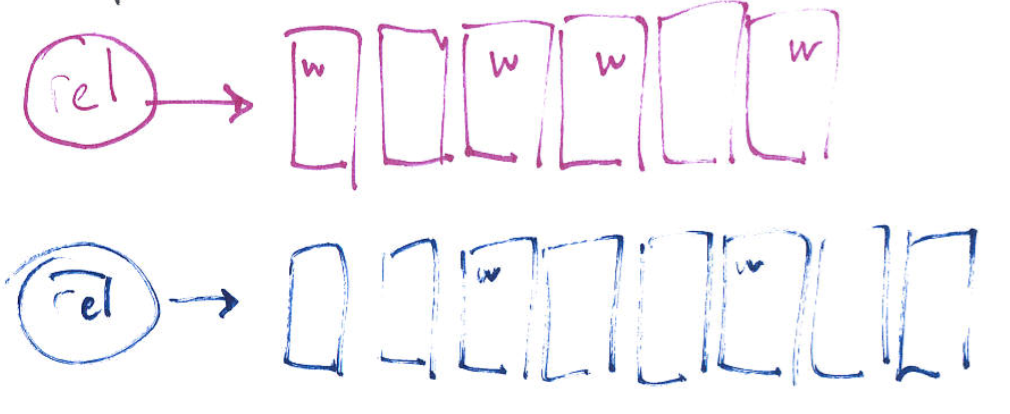
\includegraphics[width=.5\textwidth]{images/l9-fig-1}
	\caption{Dati a disposizione del modello probabilistico}\label{fig:data-prob}
\end{figure}
